\section{The evidence profile of the inventory}
\label{sec:profile}

\begin{figure}[t]
\centering
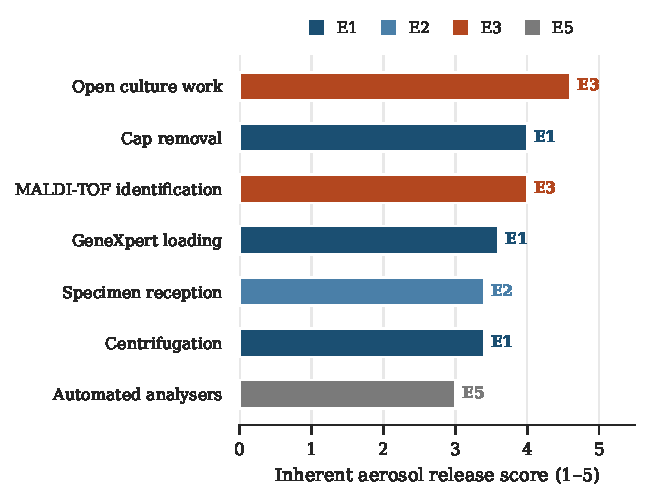
\includegraphics[width=\columnwidth]{figures/fig2_evidence_profile.pdf}
\caption{Inherent aerosol release against evidence grade for each step. Bar
length is the release score before any control is credited; colour and label
give the grade. The two steps with the highest release scores, open culture
work and MALDI-TOF target preparation, are graded E3: incident evidence
without aerosol measurement.}
\label{fig:profile}
\end{figure}

Across the seven steps the grades fall as follows: three E1, one E2, two E3,
and one E5. No step was graded E4, which is to say that no step in this
inventory rests on guidance with neither measurement nor incident evidence
behind it somewhere. Four of seven carry no direct measurement of the step
itself.

Figure~\ref{fig:profile} plots release against grade. Three features are worth
drawing out.

\subsection{The evidence runs opposite to the hazard}

The two steps with the highest release scores, open culture work at 4.6 and
MALDI-TOF target preparation at 4.0, are both graded E3. Both are supported by
incident investigations documenting real human infections, including eight
deaths in one series \cite{sejvar2005}, and neither has ever been measured
with an air sampler in a clinical laboratory.

Meanwhile the steps that have been measured, tube opening and closed-cap
centrifugation, returned negative results and sit at the bottom of the
inventory for residual biorisk at their primary profile.

The inversion is a property of how the evidence base was assembled rather than
of the hazards themselves. Measurement studies went where measurement was
tractable: a spiked surrogate in a chemistry laboratory, a simulated accident
in a containment suite. Incident investigations went where people were harmed.
These are different selection processes, and neither was aiming at a
representative picture of bench work. The result is an evidence base whose
density is unrelated to where the risk is.

\subsection{Most of the inventory is conditional}

Six of the seven steps carry a conditionality flag. Three are
failure-conditional and three technique-conditional. Only open culture work is
hazardous as correctly performed.

This matters for how a laboratory reads a recommendation. For a
failure-conditional step, controls that constrain the routine operation are
largely wasted and controls that detect and contain failure are what pay. For a
technique-conditional step, the measured reassurance is contingent on a
practice that may or may not be followed on a busy afternoon, and competency
assessment stops being a formality and becomes the control itself.

A laboratory that applies cabinet-level controls to routine centrifugation
while leaving its breakage response undefined, or that cites the negative
measurement for tube opening while permitting stoppers to be pulled with a
snap, has read the evidence without reading its conditions.

\subsection{The largest gap is at the highest throughput}

The operation of automated chemistry and haematology analysers is graded E5.
It is also, by a wide margin, the step through which the largest number of
specimens passes.

This is the clearest research priority the inventory identifies. A single well
designed measurement study on one high-volume analyser, covering normal running
and the cover-open jam and maintenance conditions separately, would move this
row from E5 to E1 and would be citable by every non-waived laboratory in the
country. No such study was located.

\subsection{Agent profile changes the picture more than any control}

The scores in Table~\ref{tab:inventory} are shown at two agent profiles because
the difference between them exceeds the difference any control set makes.

Specimen reception scores 5.67 against a bloodborne profile and 15.87 against a
low-dose inhalational profile, moving from Moderate to High on identical
release and control scores. Cap removal moves from 6.33 to 17.73. The step did
not change; what changed is the assumption about what might be in the tube.

This has a direct operational consequence. The agents that cause
laboratory-acquired infection in clinical settings are overwhelmingly those
that arrived unflagged, which means the inhalational column, not the primary
column, is the one that applies at the moment the specimen is handled. A
laboratory that assesses its pre-analytical bench against a bloodborne profile
is assessing it against the specimens it knows about.
